\documentclass[lettersize,journal]{IEEEtran}
\usepackage{amsmath,amsfonts}
\usepackage{algorithmic}
\usepackage{algorithm}
\usepackage{array}
\usepackage[caption=false,font=normalsize,labelfont=sf,textfont=sf]{subfig}
\usepackage{textcomp}
\usepackage{hyperref}
\usepackage[table,xcdraw,dvipsnames]{xcolor}
\usepackage{stfloats}
\usepackage{url}
\usepackage{verbatim}
\usepackage{graphicx}
\def\BibTeX{{\rm B\kern-.05em{\sc i\kern-.025em b}\kern-.08em
    T\kern-.1667em\lower.7ex\hbox{E}\kern-.125emX}}
\usepackage{cite}
\usepackage{booktabs}
\usepackage{glossaries}
% Enable the glossary package without hyperlinks
\glsdisablehyper

\makeglossaries
\newacronym{eca}{ECA}{Eigen-Component Analysis}
\newacronym{ueca}{uECA}{Unsupervised Eigen-Component Analysis}
% Adjusted Rand Index (ARI)
\newacronym{ari}{ARI}{Adjusted Rand Index}
\newacronym{lor}{LoR}{Logistic Regression}
\newacronym{lda}{LDA}{Linear Discriminant Analysis}
\newacronym{qda}{QDA}{Quadratic Discriminant Analysis}
\newacronym{svm}{SVM}{Support Vector Machine}
\newacronym{ksvm}{Kernel SVM}{Kernel Support Vector Machine}
\newacronym{pca}{PCA}{Principal Component Analysis}
\newacronym{rbf}{RBF}{Radial Basis Function}
\newacronym{ste}{STE}{Straight-Through Estimator}

\hyphenation{op-tical net-works semi-conduc-tor IEEE-Xplore}
% updated with editorial comments 8/9/2021

\begin{document}

\title{Eigen-Component Analysis: A Quantum-Inspired Framework\\for Feature Extraction and Classification}
\author{}

\author{\IEEEauthorblockN{Rongzhou Chen\textsuperscript{1,*}, Yaping Zhao\textsuperscript{1,*}, Haohan Xu\textsuperscript{2,*}, Hanghang Liu\textsuperscript{2},  Shaohua Ma\textsuperscript{2,3,\dag}, Edmund Y. Lam\textsuperscript{1,\dag}}
\IEEEauthorblockA{\textit{\textsuperscript{1}Department of Electrical and Electronic Engineering, The Univerisity of Hong Kong, Hong Kong SAR of China} \\
\textit{\textsuperscript{2}Tsinghua Shenzhen International Graduate School, Tsinghua University, Shenzhen, China}\\
\textit{\textsuperscript{3}Tsinghua-Berkeley Shenzhen Institute, Shenzhen, China}\\
\textsuperscript{*}Co-first author %\\ 
\textsuperscript{\dag}Corresponding author\\
\texttt{
% \{lachen,zhaoyp\}@connect.hku.hk\\
shaohua.ma@sz.tsinghua.edu.cn,
elam@eee.hku.hk}}
}

% % The paper headers
% \markboth{Journal of \LaTeX\ Class Files,~Vol.~14, No.~8, August~2021}%
% {Shell \MakeLowercase{\textit{et al.}}: A Sample Article Using IEEEtran.cls for IEEE Journals}

% \IEEEpubid{0000--0000/00\$00.00~\copyright~2021 IEEE}
% % Remember, if you use this you must call \IEEEpubidadjcol in the second
% % column for its text to clear the IEEEpubid mark.

\maketitle

\begin{abstract}
In modern machine learning circuits and systems, the need for centralized, standardized data poses significant challenges, especially in privacy-sensitive, resource-constrained, real-time, or asynchronous environments. We introduce \Gls{eca}, a quantum-inspired linear model that circumvents these requirements by leveraging intrinsic data structures. \Gls{eca} uses an orthogonal transformation to extract meaningful features from decentralized, non-standardized data, ensuring high classification accuracy without extensive preprocessing. Unlike traditional linear models, \Gls{eca} adapts to complex data distributions and shows superior performance in feature extraction and classification across various datasets. Experiments indicate that \Gls{eca} achieves robust accuracy with fewer parameters, highlighting its potential where data centralization and standardization are impractical. 
% Our work extends the feasibility of linear models in diverse scenarios, enhancing interpretability and efficiency in challenging data environments.
Moreover, we provide a theoretical explanation for the inherent sparsity in the eigenfeatures learned by \Gls{eca}, drawing on principles of energy compaction and quantum measurement theory. Our contributions extend the feasibility of linear models in a wide range of challenging data environments, enhancing both interpretability and efficiency.
The implementation of \gls{eca} is available at 
\href{https://github.com/lachlanchen/eca}{\texttt{https://github.com/lachlanchen/eca}}.
\end{abstract}

\begin{IEEEkeywords}
Distributed Learning,
Quantum-Inspired Algorithms,
Linear Models, Feature Extraction, Classification
\end{IEEEkeywords}

\section{Introduction}
\IEEEPARstart{I}{n} modern circuits and systems with complex data structures, effective feature extraction and classification pose critical challenges in machine learning~\cite{labrinidis2012challenges}. A fundamental problem is finding optimal methods to achieve high linear separability, essential for accurate classification across domains~\cite{hastie2009elements}. Conventional linear classifiers like \Gls{lor} and \Gls{lda} perform well under conditions where data are centralized, standardized, and follow simple, linearly separable distributions~\cite{hastie2009elements}. However, real-world data often violate these assumptions due to privacy restrictions, decentralization, and non-uniform distributions, necessitating approaches to handle these complexities while preserving data integrity and interpretability~\cite{yang2020federated,kaissis2020secure,li2021survey}.
Achieving reliable classification without centralized and standardized data is both crucial and challenging. In distributed or privacy-sensitive environments, such as healthcare and finance, aggregating data can be infeasible due to regulatory and logistical constraints~\cite{kaissis2020secure,li2021survey}. Additionally, non-standardized data with intricate structures often leads traditional linear models to fail, as they rely heavily on assumptions of uniformity and centralized processing~\cite{singh2020investigating}. Addressing these issues requires a method that handles distributed data while minimizing preprocessing like standardization, ensuring that classification models remain adaptable to dynamic, resource-constrained settings without sacrificing accuracy or interpretability.

Researchers have attempted to address these issues through various approaches. Some rely on dimensionality reduction techniques like \Gls{pca} or \Gls{lda}, which effectively condense data but are limited by their dependence on centralized, standardized inputs~\cite{hastie2009elements}. Others, such as \Gls{qda} and \Gls{svm}, offer better flexibility with non-linearity but tend to be computationally expensive and parameter-heavy, making them unsuitable for low-resource environments or real-time applications~\cite{pavlov2000scaling}. While these techniques perform well under controlled conditions, they often struggle with decentralized and heterogeneous datasets, limiting their scalability and practical applicability in complex real-world tasks~\cite{li2021survey}.

To address these limitations, we propose Eigen-Component Analysis (ECA), a linear model inspired by quantum theory~\cite{tang2019quantum}. \Gls{eca} introduces an orthogonal transformation that enables meaningful feature extraction from distributed, non-standardized data~\cite{sanchez1996use,kanjilal1995application,yen1999simplifying}. By leveraging the structural properties within the data, \Gls{eca} circumvents the need for centralization or standardization, ensuring that classification occurs accurately across decentralized and diverse datasets. Our approach uses orthogonal transformations to map data into a feature space where class separability is maximized~\cite{sanchez1996use,kanjilal1995application}. Experiments demonstrate that \Gls{eca} outperforms traditional methods in accuracy and requires fewer parameters, showcasing its potential in real-world applications.

We further broaden the scope of our work in two significant directions. First, we introduce an unsupervised variant of the ECA framework, termed \Gls{ueca}, which operates without explicit class labels by leveraging pairwise similarity relationships within the data to partition it into coherent clusters. This extension demonstrates the versatility of our orthogonal transformation approach in both supervised and unsupervised settings. Second, we provide a theoretical explanation for the inherent sparsity observed in the eigenfeatures learned by ECA. Drawing on the principles of energy compaction and quantum measurement theory, our analysis elucidates how the orthogonal transformation naturally concentrates discriminative information into a small subset of features while suppressing redundant ones.


Our main contributions are as follows:

\begin{itemize}
\item We propose \Gls{eca}, a quantum-inspired model for linear separability, effectively addressing the limitations of decentralized, non-standardized, undersampled, and asynchronous data in real-world settings.

\item We develop a robust orthogonal transformation that captures intrinsic data structures, enabling feature extraction without centralization or standardization.
% and enhancing model adaptability to diverse datasets.

\item Experiments show \Gls{eca} beats traditional classifiers, superior for complex data and resource-limited environments.
\item We extend the framework by introducing \Gls{ueca}, an unsupervised variant that leverages pairwise similarity relationships to partition unlabeled data into coherent clusters, demonstrating the versatility of our orthogonal transformation approach beyond supervised tasks.
\item We provide a theoretical explanation for the inherent sparsity observed in the eigenfeatures of ECA based on energy compaction and quantum measurement theory, elucidating how the orthogonal transformation naturally concentrates discriminative information while suppressing redundant features.

\end{itemize}


\section{Methods}
We develop a classification framework inspired by quantum mechanics~\cite{ciliberto2018quantum, schuld2015introduction}, aiming to find a transformation matrix \( P \) that maps input data into a space where each class corresponds to a distinct group of features represented by a mapping matrix \( L \). This section details the derivation of our method, starting from the problem formulation and leading to a practical algorithm implementable on classical computers.
\subsection{Problem Formulation}
Given a dataset \( \{ (\mathsf{x}^{(i)}, y^{(i)}) \}_{i=1}^n \), where \( \mathsf{x}^{(i)} \in \mathbb{R}^m \) is the input vector and \( y^{(i)} \in \{1, 2, \dots, l\} \) is its class label, our goal is to find an orthogonal transformation \( P \in \mathbb{R}^{m \times m} \) such that the transformed features \( \psi^{(i)} = P^\top \mathsf{x}^{(i)} \) can effectively discriminate between classes. The association between transformed features and classes is captured by a mapping matrix \( L \in [0,1]^{m \times l} \), where \( L_{jk} \) represents the degree of association between the \( j \)-th eigenfeature and class \( k \).

\subsection{Orthogonal Transformation}

To ensure that the transformation preserves the structure of the data, we require \( P \) to be orthogonal, i.e., \( P^\top P = I \), where \( I \) is the identity matrix. We achieve this by parametrizing \( P \) using the exponential of an antisymmetric matrix \( A \)~\cite{absil2008optimization}
\begin{equation}
P = e^{A},
\end{equation}
where \( A \in \mathbb{R}^{m \times m} \) satisfies \( A^\top = -A \). This parametrization ensures that \( P \) remains orthogonal during optimization.

\Gls{eca} adopts a divide-and-conquer strategy by decomposing the multi-class classification problem into multiple binary classification problems at the level of eigenfeatures~\cite{dietterich2000ensemble}. We consider each eigenfeature independently to determine its association with each class.

The mapping matrix \( L \) indicates whether an eigenfeature contributes to a particular class. We relax the binary constraint and allow \( L_{jk} \) to take continuous values in the interval \( (0,1) \), representing the probability of association~\cite{liu2011defense}.

\subsection{Class Probability Estimation}

Given an input vector \( \mathsf{x}^{(i)} \), we obtain the transformed features \( \psi_j^{(i)} = P^\top \mathsf{x}^{(i)} \) using the orthogonal transformation \( P = e^A \). Each transformed feature \( \psi_j^{(i)} \) corresponds to projections of the input data on each eigenfeature.

We compute the probability of \( \mathsf{x}^{(i)} \) belonging to class \( k \) by summing the weighted contributions of all eigenfeatures
\begin{align}
    p_k^{(i)} = \sum_{j=1}^m |\psi_j^{(i)}|^2 L_{jk},
    \label{eq:map_matrix}
\end{align}
where \( |\psi_j^{(i)}|^2 \) represents the magnitude squared of the \( j \)-th transformed feature, and \( L_{jk} \) is the degree of association between the \( j \)-th eigenfeature and class \( k \). This mirrors the concept of probability amplitudes in quantum mechanics, where the magnitude squared of the amplitude reflects the likelihood of a particular state~\cite{nielsen2010quantum}.

\subsection{Objective Function}

To derive the objective function, we aim to maximize the likelihood of the observed class labels \( y^{(i)} \) for each input \( \mathsf{x}^{(i)} \). We model the likelihood of observing the true class label \( y^{(i)} \) for a given sample as the product of the estimated class probabilities
\begin{align}
    \mathcal{L}(\theta; \mathsf{x}, \mathsf{y}) = \prod_{i=1}^{n} \prod_{k=1}^{l} p_k^{(i)}{}^{y_k^{(i)}},
\end{align}
where \( y_k^{(i)} = 1 \) if the input belongs to class \( k \), and \( 0 \) otherwise. Taking the logarithm of the likelihood, we obtain
\begin{align}
    \log \mathcal{L}(\theta; \mathsf{x}, \mathsf{y}) = \sum_{i=1}^{n} \sum_{k=1}^{l} y_k^{(i)} \log p_k^{(i)}.
\end{align}
Since we wish to minimize the negative log-likelihood, the final objective function becomes the cross-entropy loss~\cite{bilmes1998gentle}
\begin{align}
    \mathcal{J}(A, L) = -\sum_{i=1}^{n} \sum_{k=1}^{l} y_k^{(i)} \log p_k^{(i)}.
\end{align}

We optimize the parameters \( A \) and \( L \) to minimize this loss. The orthogonal transformation \( P = e^A \) ensures that the transformation matrix remains valid, preserving the structure of the input data during optimization. We learn the association matrix \( L \), bounded within \( (0,1) \), using a sigmoid function to ensure probabilistic interpretation.

\subsection{Optimization Constraints}

The optimization problem is constrained by
\begin{equation}
\begin{aligned}
P &= e^{A}, \quad A = A_{\text{raw}} - A_{\text{raw}}^\top, \quad L_{jk} \in (0,1),\\
% D &= \operatorname{diag}(d), \quad L_{jk} \in (0,1).
\end{aligned}
\end{equation}
% We ensure \( P \) remains orthogonal during optimization by updating the trainable parameters \(A_{\text{raw}}\) and \(D\), then computing \( A \) and \( P \) accordingly~\cite{hu2020brief}.
where $A$ is an anti-symmetric matrix ensuring orthogonality of the transformation. The transformation matrix $P$ incorporates a diagonal term $e^{\epsilon D}$ that preserves the orthogonality between feature vectors while providing feature-specific scaling~\cite{hu2020brief}%In our implementation, we added a modest diagonal scaling term $e^{\epsilon D}$  for additional flexibility while maintaining orthogonality between feature vectors~\cite{hu2020brief}.
% Where $A_{\text{skew}}$ is an anti-symmetric matrix yielding orthogonality, and $\epsilon D$ provides controlled feature-specific scaling via the diagonal matrix $D$. The product maintains orthogonality between feature vectors, with $\epsilon$ acting as a regularization parameter. 
%balancing strict orthonormality (as $\epsilon \rightarrow 0$) and model flexibility. 

We keep the entries of \( L \) within \( (0,1) \) using a sigmoid function
\begin{equation}
L_{jk} = \sigma(\tilde{L}_{jk}) = \frac{1}{1 + e^{-\tilde{L}_{jk}}},
\end{equation}
where \( \tilde{L}_{jk} \) are the unconstrained parameters.
%optimized during training.
We adopt a \Gls{ste}~\cite{bengio2013estimating} to approximate gradients to binarize or apply discrete constraints to \(L\). This approach enables gradient flow through the thresholding operation, allowing \(L\) to remain interpretable while still being optimized using standard backpropagation techniques.

\subsection{Unsupervised Eigen-Component Analysis}

While our primary focus is on supervised learning scenarios, we also explore an unsupervised variant of the \gls{eca} framework that operates without explicit class labels during training. This extension, termed \gls{ueca}, demonstrates the versatility of orthogonal transformations for data analysis tasks beyond supervised classification.

\subsubsection{Problem Formulation}

Given an unlabeled dataset $\{\mathsf{x}^{(i)}\}_{i=1}^n$ where $\mathsf{x}^{(i)} \in \mathbb{R}^m$, \gls{ueca} aims to discover an orthogonal transformation $P \in \mathbb{R}^{m \times m}$ and a mapping matrix $L \in [0,1]^{m \times K}$ that partition the data into $K$ coherent clusters. Similar to supervised \gls{eca}, we maintain the orthogonality constraint on $P$ by parameterizing it as $P = e^A$, where $A$ is antisymmetric.

\subsubsection{Similarity-Based Objective}

Without class labels to guide the optimization process, \gls{ueca} relies on pairwise similarity relationships within the data. We define a cosine similarity matrix $S$ where $S_{ij}$ represents the cosine similarity between normalized input vectors
\begin{equation}
S_{ij} = \frac{\mathsf{x}^{(i)^{\top}} \mathsf{x}^{(j)}}{\|\mathsf{x}^{(i)}\| \cdot \|\mathsf{x}^{(j)}\|}
\end{equation}
The objective function minimizes the sum of weighted dissimilarities, where the weighting is determined by the similarity of cluster assignments
\begin{equation}
\mathcal{J}(A, L) = \sum_{i=1}^n \sum_{j=1}^n (1 - S_{ij}) \cdot \text{sim}(p^{(i)}, p^{(j)})
\end{equation}
Here, $p^{(i)} = \text{softmax}(\mathsf{x}^{(i)}P^{\top}  L)$ represents the cluster assignment probabilities for input $\mathsf{x}^{(i)}$, and $\text{sim}(p^{(i)}, p^{(j)}) = p^{(i)^{\top}} p^{(j)}$ measures the similarity between probability distributions.

This formulation encourages inputs with high cosine similarity to have similar cluster assignments, while allowing dissimilar inputs to be assigned to different clusters. The orthogonal transformation $P$ learns to map the data into a feature space where these relationships are preserved and enhanced.

% \subsubsection{Implementation and Evaluation}

% The optimization problem remains constrained similarly to supervised \gls{eca}:
% \begin{equation}
% P = e^{A}, \quad A = A_{\text{raw}} - A_{\text{raw}}^{\top} + \text{diag}(D), \quad L_{jk} \in (0,1)
% \end{equation}

For evaluation purposes, we employ the Hungarian algorithm to determine the optimal matching between discovered clusters and ground truth classes, enabling quantitative assessment via the \gls{ari}.

% Running on dataset: iris
% UnsupervisedEigenComponentAnalysis ARI: 0.9222
% KMeans ARI: 0.9039
% Agglomerative Clustering ARI: 0.8857
% Mean Shift ARI: 0.5681


Our preliminary investigations indicate that \gls{ueca} achieves competitive clustering performance compared to traditional methods such as K-means and Mean Shift, particularly in scenarios where the data exhibit complex structural relationships. 
% While not consistently outperforming specialized clustering algorithms across all datasets, 
\Gls{ueca} offers unique advantages through its orthogonal transformation approach, which preserves distances and angles in the transformed space, potentially enhancing interpretability.

% elegance --> potential?
The elegance of \gls{ueca} lies in its unified mathematical framework with supervised \gls{eca}, highlighting how principles inspired by quantum mechanics can be effectively applied across the spectrum of learning paradigms. This extension further demonstrates the versatility of eigenfunction-based approaches for extracting meaningful structure from high-dimensional data, with or without explicit supervision.

\subsection{Implementation Details}

We implement the \Gls{eca} model using PyTorch~\cite{baydin2018automatic}, leveraging automatic differentiation and optimization tools. We define the antisymmetric matrix \( A \) as trainable parameters and compute the orthogonal transformation matrix \( P = e^{A} \) using the matrix exponential. To ensure \( L \) remains in \( (0, 1) \), we use a sigmoid activation function on its raw parameters \( \tilde{L} \).

We train the model using the Adam optimizer with a learning rate of \( 0.01 \).
% , minimizing the cross-entropy loss between the predicted class probabilities and the true labels. 
Training is performed over 1000 epochs.
The implementation of \gls{eca} is available at 
\href{https://github.com/lachlanchen/eca}{\texttt{https://github.com/lachlanchen/eca}}.


% \subsection{Interpretability}

% By analyzing the learned mapping matrix \( L \), we can interpret which eigenfeatures are most influential for each class~\cite{rudin2019stop, linardatos2020explainable}. This enhances the model's transparency and provides insights into the underlying data structure.

\subsection{Interpretability}

The interpretability of the \Gls{eca} model arises from the mapping matrix $ L $, which shows the association between eigenfeatures and classes. Each entry  $L_{jk}$  quantifies the $j$-th eigenfeature's influence on class $k$, providing insights into data structure and feature relevance for classification.

\subsection{Convergence Analysis}


\begin{figure}[ht]
    \centering
    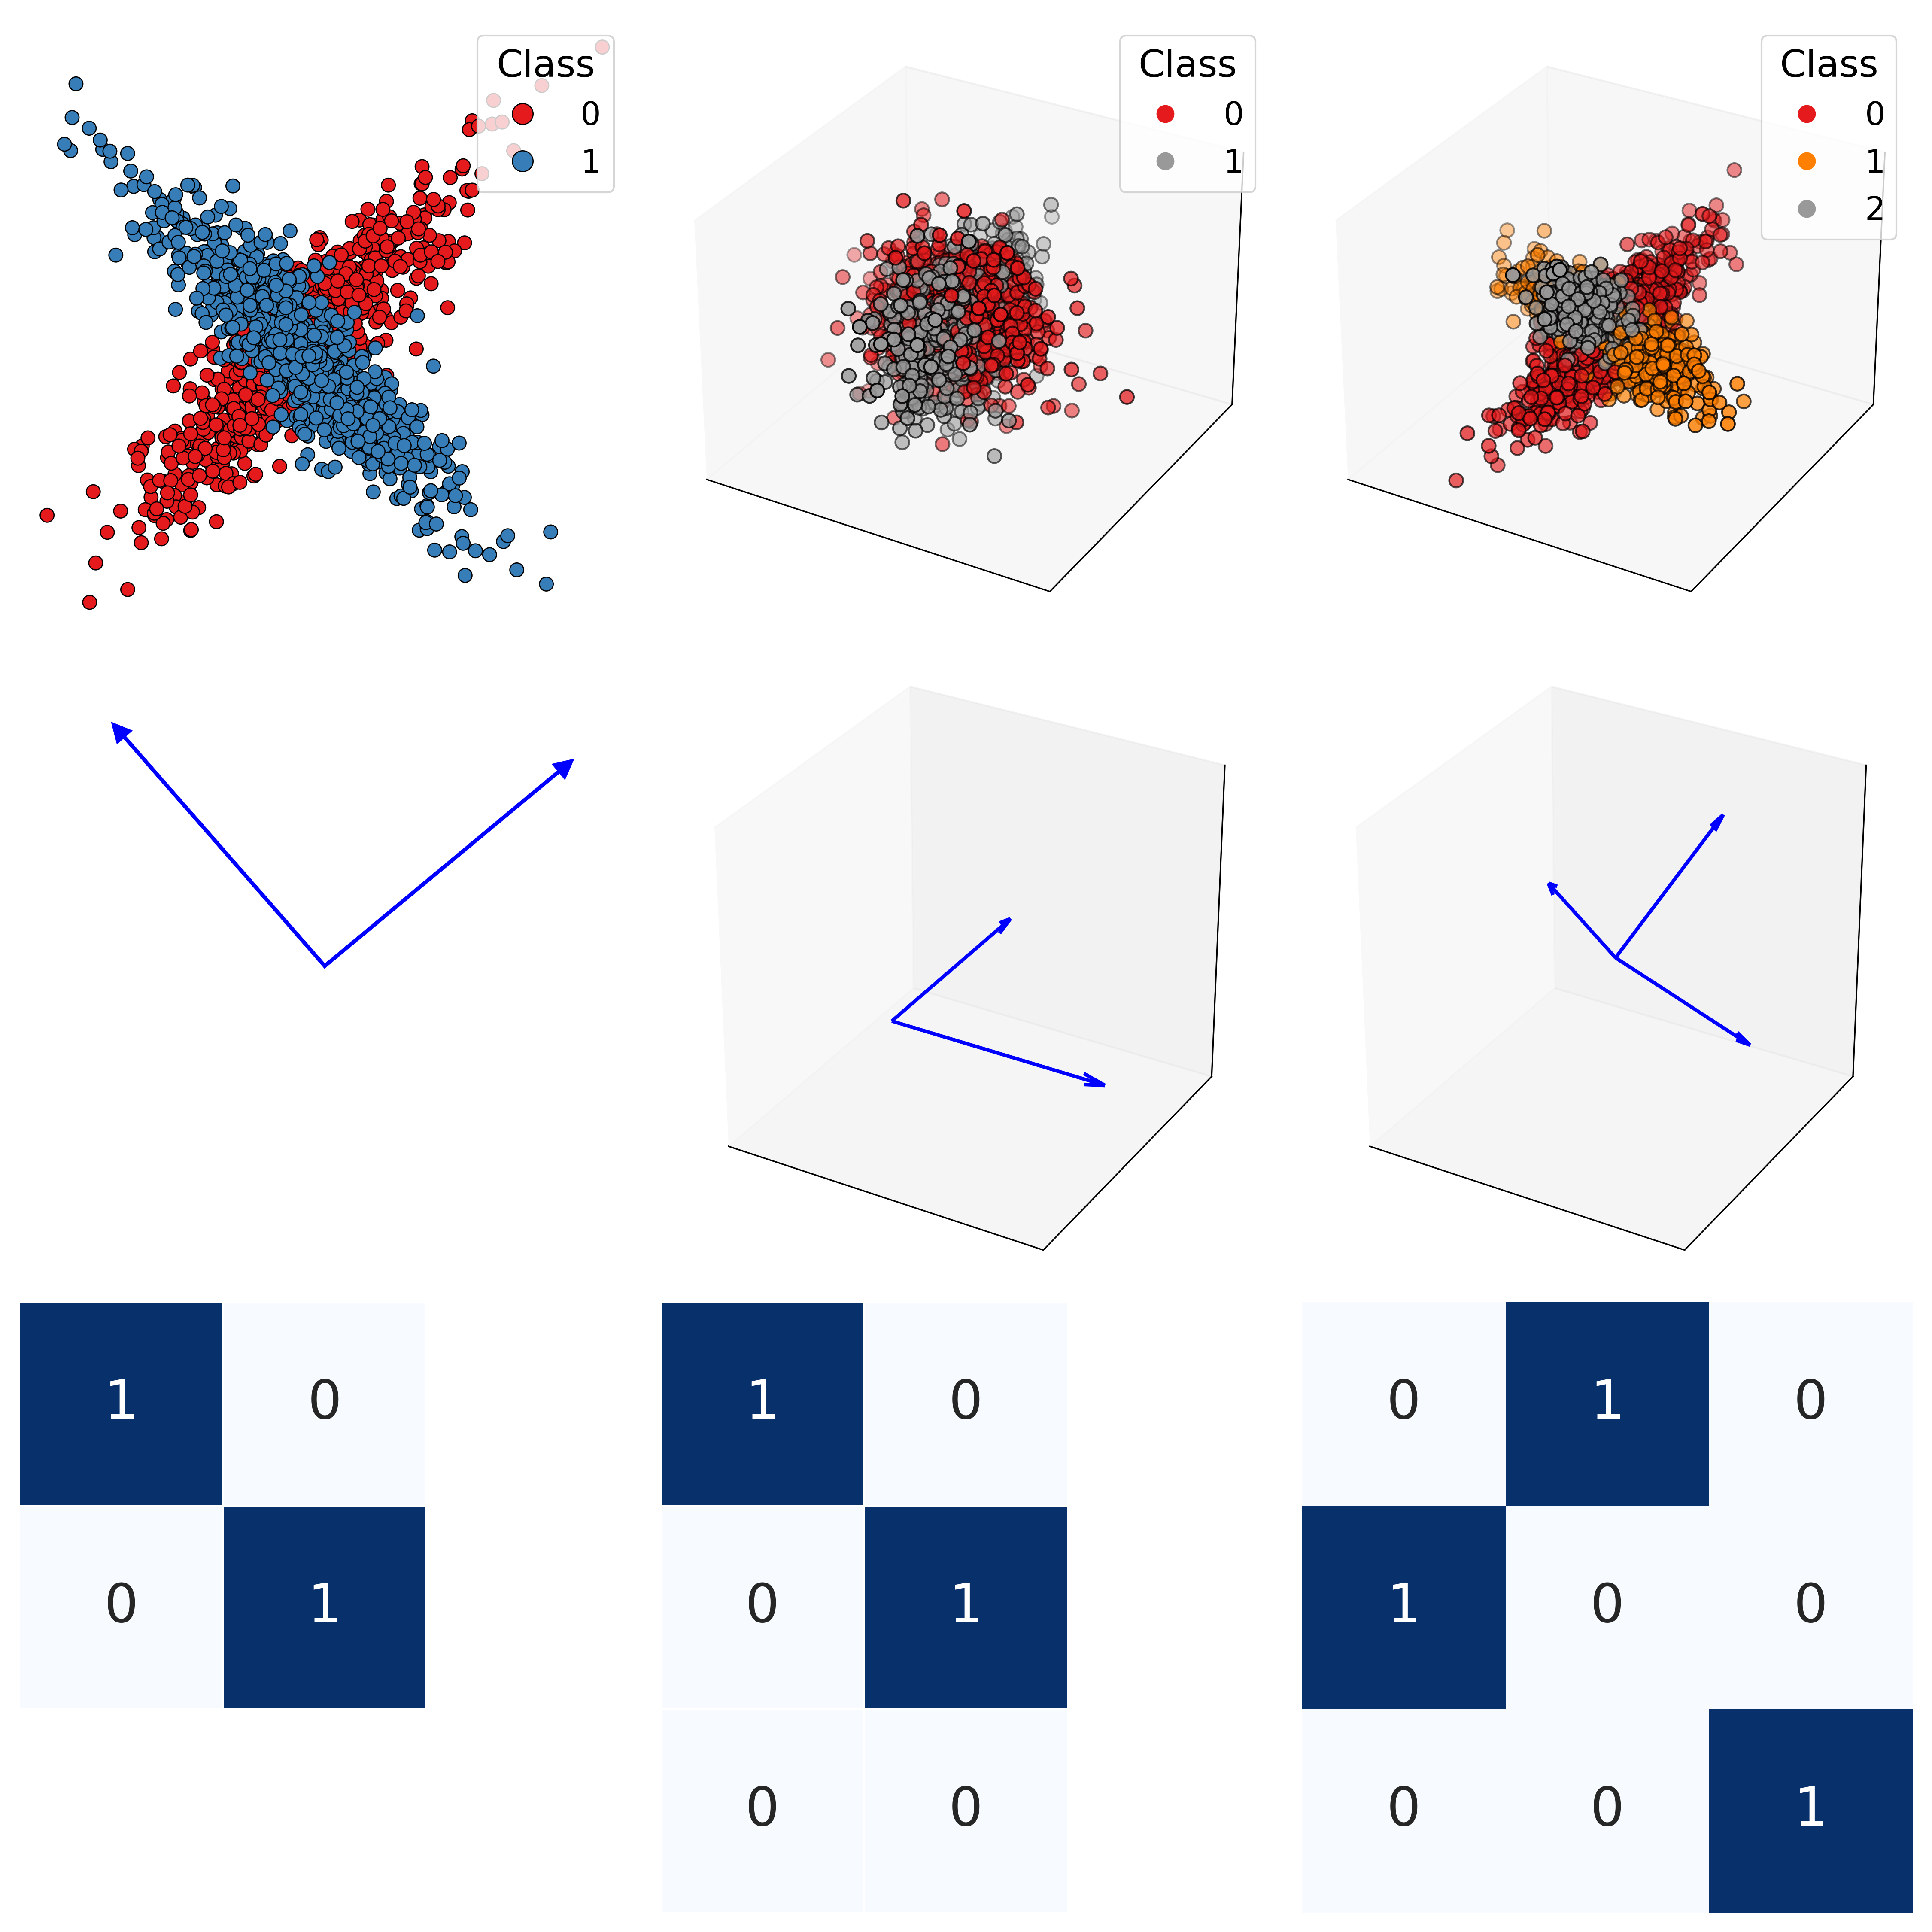
\includegraphics[width=0.9\linewidth]{figs/fig1.png}
    \caption{Visualization of the synthetic 2D and 3D datasets.}
    \label{fig:2d_3d_results}
\end{figure}

\begin{figure}[ht]
    \centering
    \includegraphics[width=0.9\linewidth]{figs/fig2_v3.png}
    \caption{Visualization of the learned transformation matrix \( e^{A} \) (top row) and mapping matrix \( L \) (bottom row) for the synthetic datasets using \Gls{eca}.}
    \label{fig:synthetic_p_l}
\end{figure}

\subsection{Sparsity Explanation Based on Energy Compaction and Quantum Measurement Theory}
\label{sec:explanation}
In the ECA framework, given an input sample 
$
\mathsf{x}^{(i)} \in \mathbb{R}^m,
$
we apply an orthogonal transformation defined by
$
P = e^A, \quad \text{with} \quad A^\top = -A,
$
to obtain the projected coefficients
$
\psi^{(i)} = P^\top \mathsf{x}^{(i)}.
$
Due to the orthogonality of \(P\) (i.e., \(P^\top P = I\)), energy is conserved:
\begin{align}
\|\mathsf{x}^{(i)}\|_2^2 = \|\psi^{(i)}\|_2^2 = \sum_{j=1}^{m} |\psi_j^{(i)}|^2.
\end{align}
If the data intrinsically lies on a low-dimensional manifold, most of the energy (or variance) of \(\mathsf{x}^{(i)}\) will be concentrated in only a few components of \(\psi^{(i)}\). This phenomenon is known as \emph{energy compaction}.

\subsubsection{Quantum Measurement Analogy}

In quantum mechanics, the squared magnitude \( |\psi_j^{(i)}|^2 \) of a projection coefficient is interpreted as the probability of measuring the system in the corresponding eigenstate (according to the Born rule). By analogy, in the ECA framework, the quantity \( |\psi_j^{(i)}|^2 \) can be seen as the ``measurement probability'' of the \(j\)-th eigenfeature being activated for sample \(i\). Consequently, if only a few eigenfeatures capture the intrinsic structure of the data, then only these features will have significant \( |\psi_j^{(i)}|^2 \) values, while the remaining coefficients are nearly zero.

\subsubsection{Role of the Mapping Matrix \(L\)}

The mapping matrix 
$
L \in [0,1]^{m \times l}
$
serves to associate each eigenfeature with the corresponding class. The predicted probability for sample \(i\) to belong to class \(k\) is given by Equation~\ref{eq:map_matrix}.
During training, the cross-entropy loss forces the model to adjust \(L\) such that only those eigenfeatures that significantly contribute (i.e., have high \( |\psi_j^{(i)}|^2 \)) are assigned substantial weights for the correct class. This mechanism naturally suppresses the contribution of irrelevant or redundant features, leading to an \emph{effective sparsity} in the feature space.


\section{Results}

To demonstrate the effectiveness and interpretability of ECA, we compare it with traditional classifiers on datasets including synthetic 2D and 3D datasets, the Iris dataset~\cite{fisher1936use}, the Digits dataset~\cite{alpaydin1998optical}, MNIST~\cite{lecun1998gradient}, and the Fashion MNIST~\cite{xiao2017fashion} datasets. We compare our model with \Gls{lor}, \Gls{lda}, \Gls{qda}, \Gls{svm}, and \Gls{ksvm} using the \Gls{rbf} kernel~\cite{hastie2009elements,cortes1995support,burges1998tutorial}.

\subsection{Synthetic Datasets}

We evaluate our method on synthetic datasets designed to challenge linear classifiers due to overlapping features and covariance structures. The datasets include a 2D dataset with two classes, a 3D dataset with two classes, and a 3D dataset with three classes (see Figure~\ref{fig:2d_3d_results}).

In the 2D dataset, \Gls{eca} achieves an accuracy of \textbf{86.00\%}, outperforming others. The learned mapping matrix \( L \) associates each eigenfeature with a specific class, effectively capturing the class distinctions. The transformation matrix \( P \) finds the optimal rotation to enhance class separability (see Figure~\ref{fig:synthetic_p_l}).

In the 3D dataset with two classes, \Gls{eca} achieves an accuracy of \textbf{74.33\%}. The model associates the first two eigenfeatures with the two classes, while the third eigenfeature is not associated with any class. This indicates that \Gls{eca} identifies and discards the irrelevant feature, enhancing classification.

In the 3D dataset with three classes, \Gls{eca} achieves an accuracy of \textbf{73.50\%}. The mapping matrix \( L \) correctly associates each eigenfeature with one of the three classes, demonstrating \Gls{eca}'s capability in multiclass scenarios.

\begin{table}[ht]
    \caption{Comparison of Classifiers on Synthetic Datasets}
    \centering
    \begin{tabular}{@{}lccc@{}}
        \toprule
        \textbf{Dataset} & \textbf{Model} & \textbf{Accuracy (\%)} & \textbf{Parameters} \\ \midrule
        2D & \Gls{lor} & 53.00 & 3 \\
        2D & \Gls{lda} & 52.33 & 3 \\
        2D & \Gls{qda} & 84.67 & 14 \\
        2D & \Gls{svm} & 56.33 & 3 \\
        2D & \Gls{ksvm} & 83.33 & 461 \\
        2D & \Gls{eca} & \textbf{86.00} & 9 \\ \midrule
        3D (2 classes) & \Gls{lor} & 49.67 & 4 \\
        3D (2 classes) & \Gls{lda} & 49.67 & 4 \\
        3D (2 classes) & \Gls{qda} & 71.67 & 26 \\
        3D (2 classes) & \Gls{svm} & 48.67 & 4 \\
        3D (2 classes) & \Gls{ksvm} & 70.00 & 774 \\
        3D (2 classes) & \Gls{eca} & \textbf{74.33} & 15 \\ \midrule
        3D (3 classes) & \Gls{lor} & 34.00 & 12 \\
        3D (3 classes) & \Gls{lda} & 33.83 & 12 \\
        3D (3 classes) & \Gls{qda} & 72.17 & 39 \\
        3D (3 classes) & \Gls{svm} & 47.33 & 12 \\
        3D (3 classes) & \Gls{ksvm} & 71.83 & 1,154 \\
        3D (3 classes) & \Gls{eca} & \textbf{73.50} & 18 \\ \bottomrule
    \end{tabular}
    \label{tab:synthetic}
\end{table}

\begin{table}[ht]
    \caption{Comparison of Classifiers on the Iris Dataset}
    \centering
    \begin{tabular}{@{}lcc@{}}
        \toprule
        \textbf{Model} & \textbf{Accuracy (\%)} & \textbf{Parameters} \\ \midrule
        \Gls{lor} & 96.67 & 15 \\
        \Gls{lda} & \textbf{100} & 15 \\
        \Gls{qda} & \textbf{100} & 63 \\
        \Gls{svm} & \textbf{100} & 15 \\
        \Gls{ksvm} & 96.67 & 49 \\
        \Gls{eca} & \textbf{100} & 26 \\ \bottomrule
    \end{tabular}
    \label{tab:iris}
\end{table}

\subsection{Iris Dataset}

We apply \Gls{eca} to the Iris dataset~\cite{fisher1936use} to evaluate its performance on a well-known multiclass classification problem with four features and three classes. Additionally, we include a comparison with \Gls{pca}~\cite{abdi2010principal} to provide context for the class separability achieved by \Gls{eca} in contrast to traditional variance-based projections. Figure~\ref{fig:iris_pca_eca} displays the visualizations of both \Gls{pca} and \Gls{eca} projections for class comparisons on the Iris dataset, illustrating separations across selected eigenfeatures for Class 1 vs. 2, Class 2 vs. 3, and Class 1 vs. 3 based on the transformation matrix \( P \).

\begin{figure*}[ht]
    \centering
    \includegraphics[width=1\linewidth]{figs/fig3_v7.png}
    \caption{Visualization of \Gls{pca} and \Gls{eca} projections for class comparisons on the Iris dataset. The figure presents a comparison between \Gls{pca} (leftmost) and \Gls{eca} projections across selected eigenfeatures, demonstrating class separations: Class 1 vs. 2 (second from left), Class 2 vs. 3 (third from left), and Class 1 vs. 3 (fourth from left), based on the transformation matrix \( P \). \Gls{pca} shows a variance-maximizing reduction, while \Gls{eca} optimizes feature space for enhanced class-specific separability. The corresponding \( L \) matrix (rightmost) highlights the association between eigenfeatures and classes, providing interpretability.}
    \label{fig:iris_pca_eca}
\end{figure*}

The \Gls{eca} model achieves an accuracy of \textbf{100\%} on the test data, matching the performance of \Gls{lda}, \Gls{qda}, and \Gls{svm}.

\subsection{Digits Dataset}

We test \Gls{eca} on the Digits dataset~\cite{alpaydin1998optical}, which consists of $8 \times 8$ images of handwritten digits (total 64 features) across ten classes. The \Gls{eca} model achieves an accuracy of \textbf{99.17\%}, outperforming \Gls{lor}, \Gls{lda}, and \Gls{svm}, and matching the performance of \Gls{ksvm}.

\begin{table}[ht]
    \caption{Comparison of Classifiers on the Digits Dataset}
    \centering
    \begin{tabular}{@{}lcc@{}}
        \toprule
        \textbf{Model} & \textbf{Accuracy (\%)} & \textbf{Parameters} \\ \midrule
        \Gls{lor} & 86.67 & 650 \\
        \Gls{lda} & 95.28 & 650 \\
        \Gls{qda} & 73.33 & 41,610 \\
        \Gls{svm} & 88.06 & 2,925 \\
        \Gls{ksvm} & \textbf{99.17} & 663 \\
        \Gls{eca} & \textbf{99.17} & 2,784 \\ \bottomrule
    \end{tabular}
    \label{tab:digits}
\end{table}

\subsection{Fashion MNIST Dataset}

We apply \Gls{eca} to the Fashion MNIST dataset~\cite{xiao2017fashion}, which consists of $28 \times 28$ grayscale images of clothing items across ten classes. We downsample the data by a factor of 100 due to convergence difficulties for traditional algorithms. The \Gls{eca} model achieves an accuracy of \textbf{80.71\%}, outperforming other linear models, while \Gls{qda} suffered from colinearity issues in the high-dimensional, raw data.

\begin{table}[ht]
    \caption{Comparison on the Downsampled Fashion MNIST Dataset}
    \centering
    \begin{tabular}{@{}lcc@{}}
        \toprule
        \textbf{Model} & \textbf{Accuracy (\%)} & \textbf{Parameters} \\ \midrule
        \Gls{lor} & 77.14 & 7,850 \\
        \Gls{lda} & 53.57 & 7,850 \\
        \Gls{qda} & 17.86 & 6,154,410 \\
        \Gls{svm} & 77.14 & 35,325 \\
        \Gls{ksvm} & 74.29 & 435 \\
        \Gls{eca} & \textbf{80.71} & 316,344 \\ \bottomrule
    \end{tabular}
    \label{tab:fashion_mnist}
\end{table}

\subsection{MNIST Dataset}

\begin{table}[ht]
    \caption{Comparison on the Downsampled MNIST Dataset}
    \centering
    \begin{tabular}{@{}lcc@{}}
        \toprule
        \textbf{Model} & \textbf{Accuracy (\%)} & \textbf{Parameters} \\ \midrule
        \Gls{lor} & 84.29 & 7,850 \\
        \Gls{lda} & 20.71 & 7,850 \\
        \Gls{qda} & 21.43 & 6,154,410 \\
        \Gls{svm} & 85.71 & 35,325 \\
        \Gls{ksvm} & 87.86 & 488 \\
        \Gls{eca} & \textbf{88.57} & 316,344 \\ \bottomrule
    \end{tabular}
    \label{tab:mnist}
\end{table}

We evaluate \Gls{eca} on the MNIST dataset~\cite{lecun1998gradient}, which consists of $28 \times 28$ grayscale images of handwritten digits across ten classes. Due to convergence difficulties for traditional methods, we downsample the data by a factor of 100 (both train and test datasets). We also compare different algorithms with varying sample rates to observe their performance trends. The \Gls{eca} model achieves an accuracy of \textbf{88.57\%}, outperforming \Gls{lor} and closely matching \Gls{svm}.

\begin{figure}[ht]
    \centering
    \includegraphics[width=0.9\linewidth]{figs/fig4_v2.png}
    \caption{Accuracy comparison on MNIST varying downsample fractions.}
    \label{fig:mnist_downsample}
\end{figure}

To further explore the robustness of \Gls{eca} over different training sample sizes, we conduct experiments by varying the downsample fraction of the training data while keeping the test data ratio fixed (0.2 of the full dataset). We downsample the training data from 48,000 samples to 48 samples.

As shown in Figure \ref{fig:mnist_downsample}, \Gls{eca} consistently outperforms \Gls{lor} and \Gls{lda}, especially at lower downsample fractions. \Gls{eca} maintains high accuracy even with significantly reduced training data, showcasing its robustness on sparse data. 
%The results for \Gls{svm} and \Gls{ksvm} at the lowest downsample rates are omitted due to convergence difficulties.

\begin{figure*}[ht]
    \centering
    \includegraphics[width=0.95\linewidth]{figs/mnist_L_heatmap_2.png}
    \caption{Heatmap of the mapping matrix $L$ for MNIST dataset. Each column represents an eigenfeature and each row corresponds to a digit class (0-9). The intensity of blue coloration indicates the strength of association between eigenfeatures and classes. The sparsity pattern demonstrates that \Gls{eca} identifies a minimal subset of eigenfeatures that efficiently represent each class while maintaining discriminative power. This visualization reveals the dimensionality reduction capabilities of \Gls{eca}, effectively encoding the data's intrinsic manifold structure through the orthogonal transformation.}
    \label{fig:mnist_L_heatmap}
\end{figure*}

\begin{figure}[ht]
    \centering
    \includegraphics[width=0.95\linewidth]{figs/eigenfeature_distribution_2.png}
    \caption{Distribution of pure and shared eigenfeatures across MNIST digit classes. Pure eigenfeatures (pink) are uniquely associated with a single class, serving as discriminative features that capture class-specific characteristics. Shared eigenfeatures (blue) contribute to multiple classes, representing common structural patterns. This heterogeneous distribution reflects the varying topological complexity of digit classes, with digit `7' requiring the most pure eigenfeatures (22) and digit `0' requiring the fewest total eigenfeatures (9). The distribution aligns with compressive sensing principles, where complex data can be efficiently represented using a small number of basis elements when the underlying structure exhibits sparsity in an appropriate domain.}
    \label{fig:eigenfeature_distribution}
\end{figure}

\begin{figure}[ht]
\centering
\includegraphics[width=0.9\linewidth]{figs/eigen-digit-soft.png}
\caption{Visualization of selected pure eigenfeatures for each digit class (0-9) extracted by the \Gls{eca} model. Each row presents five representative eigenfeatures uniquely associated with the corresponding digit class. The binary patterns represent the orthogonal projections learned through the transformation matrix $P$, capturing class-specific topological characteristics. Notably, certain eigenfeatures exhibit morphological resemblance to their associated digits (e.g., vertical strokes for class `1', circular structures for class `0'), while others capture more abstract discriminative features that maximize inter-class separability within the transformed feature space. This diverse spectrum of eigenfeatures demonstrates how \Gls{eca} learns an interpretable basis for the underlying low-dimensional manifolds of each digit class, facilitating effective dimensionality reduction while preserving essential discriminative information.}
\label{fig}
\end{figure}

\subsection{Eigenfeature Analysis of MNIST}

To investigate the efficacy of \Gls{eca} in extracting meaningful features from high-dimensional image data, we conducted an in-depth analysis of the eigenfeature distribution across the MNIST dataset. Figure~\ref{fig:mnist_L_heatmap} presents the mapping matrix $L$, which establishes the relationship between eigenfeatures (columns) and digit classes (rows). This matrix effectively encodes a low-dimensional manifold representation of the data, where each eigenfeature acts as a basis vector in the transformed feature space. The sparsity pattern observed in $L$ reveals that \Gls{eca} successfully identifies a minimal subset of eigenfeatures necessary for accurate classification while preserving the intrinsic structure of the data.

Figure~\ref{fig:eigenfeature_distribution} quantifies the distribution of pure and shared eigenfeatures across the ten digit classes. Pure eigenfeatures, which uniquely correspond to a single class, serve as discriminative features that capture class-specific characteristics. Conversely, shared eigenfeatures contribute to multiple classes and represent common structural patterns across different digits. This distribution aligns with principles from compressive sensing theory, where complex data can be efficiently represented using a small number of basis elements when the underlying structure exhibits sparsity in an appropriate domain. The heterogeneous distribution observed across digit classes reflects the varying complexity of each digit's topology. For instance, digit `7' exhibits the highest number of pure eigenfeatures (22), suggesting more unique structural patterns, while digit `0' requires the fewest eigenfeatures overall (9), indicating greater structural simplicity.

Quantitative analysis reveals that the model identified 198 significant eigenfeatures out of the 784 available dimensions (28×28 pixels), achieving a dimensionality reduction of approximately 75\% while maintaining discriminative power. This efficient representation supports the hypothesis that \Gls{eca} can effectively capture the essential variability in the data through orthogonal transformations without requiring explicit centralization or standardization. The observed pattern of eigenfeature allocation demonstrates that \Gls{eca} automatically adapts to the intrinsic complexity of each class, assigning more computational resources to digits with more complex topological structures.

To further investigate the structural patterns learned by the model, we visualize representative pure eigenfeatures for each digit class in Figure \ref{fig}. These eigenfeatures, selected from the orthogonal basis generated by the transformation matrix $P$, reveal the underlying low-dimensional manifold structures that the model exploits for classification. The visualized eigenfeatures exhibit varying degrees of topological similarity to their corresponding digits, with some capturing holistic digit-like structures while others represent distinctive sub-components or discriminative features. This heterogeneity in eigenfeature morphology corroborates the theoretical framework of manifold learning, wherein high-dimensional data can be effectively represented on lower-dimensional subspaces that preserve essential topological characteristics. The binary nature of these eigenfeatures—representing the projection of input data onto specific directions in the transformed feature space—demonstrates how \Gls{eca} decomposes complex patterns into interpretable basis elements that span the class-specific subspaces.

According to the theoretical analysis in Section~\ref{sec:explanation} and the empirical observations described above, even without employing traditional sparse regularization terms, the ECA framework inherently yields a sparse representation due to:
\begin{enumerate}
    \item \textbf{Energy Compaction:} The orthogonal transformation \(P\) redistributes the input energy such that, if the data lies on a low-dimensional manifold, only a few projection coefficients in \(\psi^{(i)}\) carry significant energy.
    \item \textbf{Quantum Measurement Analogy:} Interpreting \( |\psi_j^{(i)}|^2 \) as a probability shows that only a few eigenfeatures are effectively ``observed'' (i.e., contribute to the classification decision).
    \item \textbf{Selective Weighting by \(L\):} The mapping matrix \(L\) is trained to amplify the contribution of those eigenfeatures with high activation, while features with near-zero activations receive negligible weights. This enforces a form of sparsity in the effective features used for classification.
\end{enumerate}

% \begin{figure*}[ht]
%     \centering
%     \includegraphics[width=0.95\linewidth]{figs/ueca_iris_visualization_3d_optimized.png}
%     \caption{Unsupervised ECA applied to the Iris dataset. (left) The training loss curve demonstrates stable convergence of the optimization process, with the minimum loss achieved at approximately epoch 1500. (middle) Projection of data onto the three principal eigenfeatures discovered through orthogonal transformation, where marker shapes indicate true classes (circle: Setosa, triangle: Versicolor, square: Virginica), colors represent correct (class-specific colors) versus incorrect (red) cluster assignments, and the \gls{ari} quantifies clustering quality. Without explicit class supervision, \gls{ueca} identifies a feature space that largely respects the natural class boundaries present in the data.}
%     \label{fig:ueca_iris}
% \end{figure*}

\begin{figure*}[ht]
    \centering
    \includegraphics[width=0.95\linewidth]{figs/ueca_iris_visualization_3d_no_tick.png}
    \caption{Unsupervised ECA applied to the Iris dataset. (left) The training loss curve demonstrates stable convergence of the optimization process, with the minimum loss achieved at approximately epoch 1500. (middle) Projection of data onto the three principal eigenfeatures discovered through orthogonal transformation, where marker shapes indicate true classes (circle: Setosa, triangle: Versicolor, square: Virginica), colors represent correct (class-specific colors) versus incorrect (red) cluster assignments, and the \gls{ari} quantifies clustering quality. Without explicit class supervision, \gls{ueca} identifies a feature space that largely respects the natural class boundaries present in the data. (right) The L matrix mapping illustrates the relationship between input features and output clusters, with values indicating the strength of each connection. This mapping reveals which features are most informative for distinguishing between classes, with Sepal Length showing strong associations with Setosa and Virginica clusters, while Petal dimensions primarily drive the Versicolor cluster identification.}
    \label{fig:ueca_iris}
\end{figure*}


\subsection{Exploratory Analysis with Unsupervised ECA}

To illustrate the potential of \gls{ueca}, we conducted an exploratory analysis on the Iris dataset. While our primary focus remains on supervised learning paradigms, this preliminary investigation offers insights into the framework's versatility across learning contexts.

Figure~\ref{fig:ueca_iris} presents the results of applying \gls{ueca} to the Iris dataset without utilizing class labels during training. The visualization illustrates three key aspects of the method: (left) the convergence behavior of the loss function during training and (middle) the projection of data points onto the discovered eigenfeatures, with color and shape coding to indicate both true classes and clustering accuracy, and (right) the L matrix that reveals the mapping between input features and discovered clusters.

% Running on dataset: iris
% UnsupervisedEigenComponentAnalysis ARI: 0.9222
% KMeans ARI: 0.9039
% Agglomerative Clustering ARI: 0.8857
% Mean Shift ARI: 0.5681


The \gls{ueca} model achieved an Adjusted Rand Index of $0.92$ on the Iris dataset, indicating substantial agreement between the discovered clusters and the ground truth classes. This performance is particularly noteworthy given that the algorithm operates without access to class labels. The visualization reveals that \gls{ueca} successfully separates the Setosa class (circles) from the other two classes, while maintaining a reasonable distinction between Versicolor and Virginica despite their known overlap in feature space.

It is important to note that while \gls{ueca} demonstrates promising capabilities on this dataset, we do not position it as universally superior to established clustering techniques. Rather, its value lies in offering an alternative perspective through the lens of orthogonal transformations, potentially capturing structural relationships that might be less apparent with traditional distance-based clustering approaches. 

The eigenfeature projections suggest that \gls{ueca}'s strength may lie in its capacity to discover meaningful low-dimensional representations that align with natural class boundaries, even when those boundaries are not explicitly provided during training. This characteristic aligns with our broader thesis regarding the efficacy of quantum-inspired orthogonal transformations for uncovering intrinsic data structures.

These preliminary findings motivate further investigation into the theoretical connections between supervised and unsupervised variants of our framework, potentially leading to hybrid approaches that leverage both labeled and unlabeled data in semi-supervised learning scenarios—a direction we consider promising for future research.

\section{Conclusion}

This paper introduces \Gls{eca}, a quantum-inspired model designed to achieve linear separability without requiring data centralization or standardization. \Gls{eca} leverages a robust orthogonal transformation to capture intrinsic data structures, enabling effective feature extraction and classification even in distributed and privacy-sensitive environments. Extensive experimentation across various datasets demonstrates that \Gls{eca} consistently outperforms traditional linear classifiers, achieving high accuracy and efficiency, particularly in complex and resource-constrained settings.

\section*{Acknowledgments}
This work is supported in part by the Research Grants Council (GRF 17201822 and TRS T45-701/22-R) of Hong Kong SAR, China; and in part by Department of Science
and Technology of Guangdong Province (2023B0909020003).



% {\appendix[Proof of the Zonklar Equations]
% Use $\backslash${\tt{appendix}} if you have a single appendix:
% Do not use $\backslash${\tt{section}} anymore after $\backslash${\tt{appendix}}, only $\backslash${\tt{section*}}.
% If you have multiple appendixes use $\backslash${\tt{appendices}} then use $\backslash${\tt{section}} to start each appendix.
% You must declare a $\backslash${\tt{section}} before using any $\backslash${\tt{subsection}} or using $\backslash${\tt{label}} ($\backslash${\tt{appendices}} by itself
%  starts a section numbered zero.)}



%{\appendices
%\section*{Proof of the First Zonklar Equation}
%Appendix one text goes here.
% You can choose not to have a title for an appendix if you want by leaving the argument blank
%\section*{Proof of the Second Zonklar Equation}
%Appendix two text goes here.}
\section{REFERENCES}
\bibliographystyle{IEEEtran}
\bibliography{ref}
\vfill

\end{document}


